We propose to specify and verify a simple load balancing system with
Helena.  The full net is illustrated by
Figure~\ref{fig_load_balancer}. Initial markings and transition guards
have been omitted to clarify the figure.

\begin{figure}[!h]
\centerline{\scalebox{0.5}{ 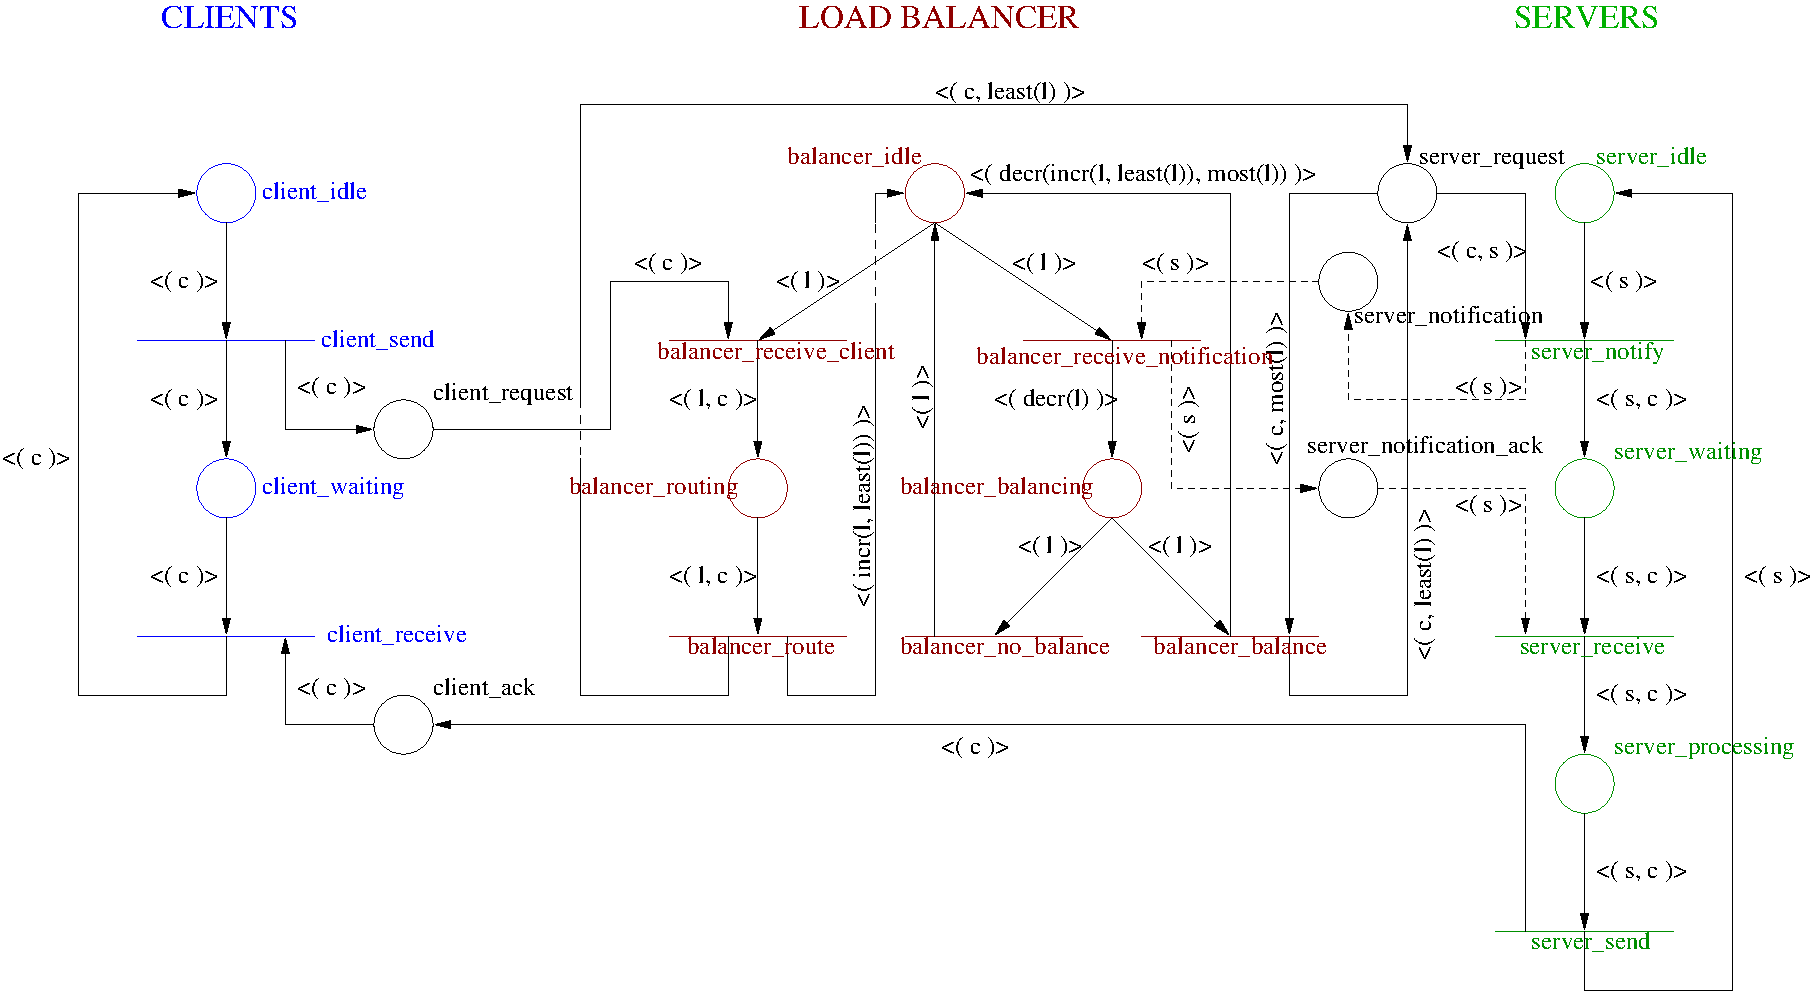
\includegraphics{load_balancer}}}
\caption{The whole load balancing system}
\label{fig_load_balancer}
\end{figure}

In this system, we have two kinds of process: a set of clients and a
set of servers. An additional process called the load balancer
distribute requests of clients to servers. Its task is also to
redistribute pending requests when servers accept requests in order to
maintain the loads of servers balanced.

\paragraph{The clients}
We note \lstinline{C} the number of clients considered. Clients are
numbered from \lstinline{1} to \lstinline{C}. The behavior of the
clients is quite simple. A client may want to send a request to a set
of servers. Instead of asking a server directly, he sends the request
to the load balancer which will route the request to the adequate
server, i.e., the least loaded server. Once the request sent, the
client waits for the answer. When this one arrives, the client comes
back to the idle state.

\paragraph{The servers}
The number of servers is noted \lstinline{S}. Servers are numbered from
\lstinline{1} to \lstinline{S}. Servers receive requests from clients via the
load balancer process. When a server accepts a request, he first has
to notify this to the load balancer process, in order that this one
rebalances the pending requests. Then he has to wait for an
acknowledgment from the load balancer to start treating the request.
Once the request treated, he directly sends the answer to the
concerned client and goes back to the idle state.

\paragraph{The load balancer}
The load balancer can perform two kinds of task. The first one is to
redirect each client request to the least loaded server. Secondly,
when a server accepts a request from a client the load balancer has to
rebalance the pending requests. If these are already balanced, the
load balancer has nothing to perform and can come back to its idle
state (transition \lstinline{balancer_no_balance}). If the loads are
not balanced, the load balancer takes a pending request of the most
loaded server and redirects it to the least loaded server (transition
\lstinline{balancer_balance}).   The load balancer has to maintain for
each server the number of requests sent to this server.

\lstinputlisting[frame=single,
caption={Helena file of the load balancing system
(file \texttt{examples/load\_balancer.lna})},
numbers=left,basicstyle=\small] {../examples/load_balancer.lna}

\lstinputlisting[frame=single,
caption={Helena file of the load balancing system properties
(file \texttt{examples/load\_balancer.prop.lna})},
numbers=left,basicstyle=\small] {../examples/load_balancer.prop.lna}
